%%%%%%%%%%%%%%%%%%%%%%%%%%%%%%%%%%%%%%%%%%%%%%%%%%%%%%%%%%%%%%%%%%%%%%%%
\chapter{Sistemi interagenti: un'introduzione}
\label{cap:interagenti}
%%%%%%%%%%%%%%%%%%%%%%%%%%%%%%%%%%%%%%%%%%%%%%%%%%%%%%%%%%%%%%%%%%%%%%%%

In questo breve Capitolo daremo una trattazione semplificata del formalismo necessario al trattamento di sistemi interagenti classici, fermandoci al caso dei gas reali e al calcolo, in prima approssimazione, dell'equazione di stato di van der Waals.

Attraverso lo studio empirico della relazione tra pressione, volume e temperatura dei gas reali, van der Vaals arrivò a un'equazione di stato fenomenologica:
\be
\label{eq:06-vanderWaals}
\left(
P + \dfrac{a}{v^2}
\right)(v-b) = kT
\ee
in cui $v = V/N$ è il volume specifico. Le quantità $a$ e $b$ sono quantità fenomenologiche, da adattare di volta in volta allo specifico gas ideale studiato. L'equazione (\ref{eq:06-vanderWaals}) è valida per un grande range di temperature, e cessa di valere solo quando siamo costretti a prendere in considerazione gli effetti quantistici (vedi Capitoli successivi). In prima approssimazione possiamo considerare $a$ e $b$ indipendenti dalla temperatura.

%%%%%%%%%%%%%%%%%%%%%%%%%%%%%%%%%%%%%%%%%%%%%%%%%%%%%%%%%%%%%%%%%%%%%%%%
\section{Espansione in cluster di un gas classico}
%%%%%%%%%%%%%%%%%%%%%%%%%%%%%%%%%%%%%%%%%%%%%%%%%%%%%%%%%%%%%%%%%%%%%%%%

Se le $N$ particelle di un gas interagiscono tra loro, possiamo scrivere, in tutta generalità,
\be
\Ham = \sum_{i=1}^{N} \dfrac{p_i^2}{2m} + \calU(r_1, r_2 \dots r_N)
\ee
Una prima approssimazione consiste nel considerare un potenziale $\calU$ che sia la somma di tutte le possibili interazioni a due corpi, descritte da un potenziale
$u_{ij}(r_{ij})$, con $i,j = 1, 2\dots N$ e $r_{ij}$ uguale al modulo del raggio vettore che unisce la coppia di particelle $(i,j)$. In questo modo abbiamo
\be
\Ham = \sum_{i=1}^{N} \dfrac{p_i^2}{2m} + \sum_{i<j} u_{ij}(r_{ij})
\ee
in cui il limite inferiore sulla seconda somma è dato dal fatto che non vogliamo contare la stessa coppia due volte. Possiamo subito scrivere la funzione di partizione totale del sistema, funzione di partizione che stavolta, in virtù delle interazioni, non può essere scritta come produttoria sulle funzioni di partizione di singola particella:
\be
Q_N(V,T) = \dfrac{1}{N!h^{3N}}\int e^{-\beta\sum_i p^2_i/2m}\,\de^{3N}p 
\int e^{-\beta\sum_{i<j}u_{ij}} \,\de^{3N}r
\ee
L'integrale sui momenti è immediato, e otteniamo
\be
Q_N(V,T) = \dfrac{1}{N!\lambda^{3N}}\int \prod_{i<j}\left(e^{-\beta u_{ij}}\right)\,\de^{3N}r \equiv \dfrac{1}{N!\lambda^{3N}}Z_N(V,T)
\ee
in cui nell'ultima abbiamo definito la quantità $Z_N(V,T)$, che è quella che ci rimane da calcolare. Introduciamo ora la quantità $f_{ij} \equiv e^{-\beta u_{ij}} - 1$. Il motivo di questa definizione può diventare chiaro se guardiamo la figura \ref{fig:06-deffij}. Nella figura abbiamo graficato un potenziale intermolecolare tipico, e in particolare il potenziale di Lennard-Jones
\be
u(r) = 4\varepsilon\left[
\dfrac{\sigma}{r^{12}} - \dfrac{\sigma}{r^{6}}
\right]
\ee
con $\varepsilon = \sigma = 1$, e la risultante funzione $f_{ij}$. Il minimo del potenziale si ottiene per un valore $r_0 = 2^{1/6}\sigma$, ed è lo stesso valore per il quale la funzione $f_{ij}$ ha un massimo. Si noti che il termine repulsivo del potenziale, proporzionale a $r^{-12}$, crea una vera e propria barriera: per $r < r_0$ sale così velocemente che difficilmente le particelle possono avvicinarsi a una distanza minore di $r_0$. 
Al contempo il termine attrattivo, proporzionale a $r^{-6}$, va a zero molto velocemente, e per valori pari a $3\sigma$ lo possiamo considerare sostanzialmente nullo. 

%%%%%%%%%%%%%%%%%%%%%%%%%%%%%%%%%%%%%%%%%%%%%%%%%%%%%%%%%%%%%%%%%%%%%%%%%
\begin{figure}[h]
  \centering
  \begin{tikzpicture}[domain={0.92:2.5},xscale=7,yscale=1]
  \draw[->] (0.8,-1.3) -- (2.5,-1.3) node[anchor=north] {$x$};
  \draw[->] (0.8,-1.3) -- (0.8,4);
  \draw[densely dotted] (0.8,0) -- (2.5,0);
  
  \draw[thick,blue,samples=100,smooth] plot[id=int-uLJ] function{4*(x**(-12)-x**(-6))};
  \draw[thick,red,samples=100,smooth,domain={0.8:2.5}]  plot[id=int-fLJ] function{exp(-4*(x**(-12)-x**(-6)))-1};

  \draw[blue] (1.0,2.6) node{$u(r)$};
  \draw[red]  (1.4,1.0) node{$f(r)$};

  \foreach \x in {0.8,1.3,1.8,2.3}
    \draw (\x cm,-1.35) -- (\x cm,-1.25) node[anchor=north] {$\x$};
  \foreach \y in {-1, 0, 1, 2}
    \draw (0.81,\y cm) -- (0.79,\y cm) node[anchor=east] {$\y$};
\end{tikzpicture}


  \caption{Potenziale di Lennard--Jones $u(r)$ con $\epsilon=\sigma=1$. Nella figura è mostrata anche la rispettiva funzione $f(r)$.}
  \label{fig:06-deffij}
\end{figure}
%%%%%%%%%%%%%%%%%%%%%%%%%%%%%%%%%%%%%%%%%%%%%%%%%%%%%%%%%%%%%%%%%%%%%%%%%

Come si vede la funzione $u_{ij}$, andando a infinito così velocemente verso l'origine, non è un buon ``parametro d'espansione''. Al contrario la funzione $f_{ij}$ è praticamente costante (e uguale a $-1$) per $r < r_0$, sale rapidamente a moderati valori positivi in un range molto limitato e poi crolla a zero velocemente; sembra quindi un buon ``parametro d'espansione'', anche se va chiarito il concetto di ``parametro d'espansione'' riferito a una funzione.
Scriviamo dunque
\bea
\label{eq:06-expaZN1}
Z_N(V,T) &=& \int \prod_{i<j}\left( 1 + f_{ij} \right)\,\de^{3N}r \nonumber \\
&=& \int \left[ 1 + \sum_{i<j}f_{ij} + \sum_{i<j<k<l} f_{ij}f_{kl} + \cdots
\right]\,\de^{3N}r
\eea
Il primo termine nella (\ref{eq:06-expaZN1}) è pari a $V^N$; il che d'altronde dovrebbe risultare ovvio, perché in assenza di interazioni (tutte le $f_{ij} = 0$) dobbiamo ritrovare l'espressione per la funzione di partizione di un gas ideale, come infatti è il caso. Il secondo termine, $\sum_{i<j} f_{ij}$, corrisponde in realtà a $N(N-1)/2$ termini, perché tale è il numero di coppie $(i,j)$ distinte che possiamo formare avendo a disposizione $N$ particelle, e così via.

%%%%%%%%%%%%%%%%%%%%%%%%%%%%%%%%%%%%%%%%%%%%%%%%%%%%%%%%%%%%%%%%%%%%%%%%%
\begin{figure}[h]
  \centering
  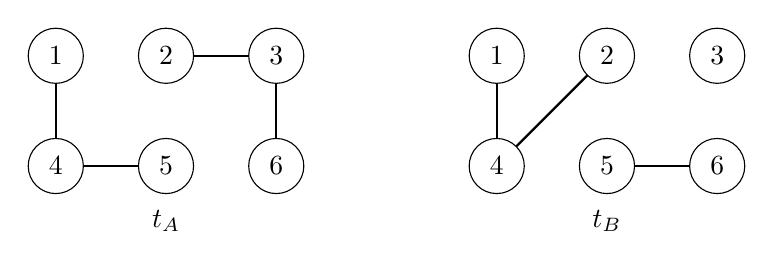
\begin{tikzpicture}[scale=0.7]

\draw ( 0,2) circle (0.5cm);
\draw ( 2,2) circle (0.5cm);
\draw ( 4,2) circle (0.5cm);
\draw ( 0,0) circle (0.5cm);
\draw ( 2,0) circle (0.5cm);
\draw ( 4,0) circle (0.5cm);

\draw ( 8,2) circle (0.5cm);
\draw (10,2) circle (0.5cm);
\draw (12,2) circle (0.5cm);
\draw ( 8,0) circle (0.5cm);
\draw (10,0) circle (0.5cm);
\draw (12,0) circle (0.5cm);

\draw ( 0,2) node{1};
\draw ( 2,2) node{2};
\draw ( 4,2) node{3};
\draw ( 0,0) node{4};
\draw ( 2,0) node{5};
\draw ( 4,0) node{6};

\draw ( 8,2) node{1};
\draw (10,2) node{2};
\draw (12,2) node{3};
\draw ( 8,0) node{4};
\draw (10,0) node{5};
\draw (12,0) node{6};

\draw[thick] (0,1.5) -- (0,0.5);
\draw[thick] (0.5,0) -- (1.5,0);
\draw[thick] (2.5,2) -- (3.5,2);
\draw[thick] (4,1.5) -- (4,0.5);

\draw[thick] (8,1.5) -- (8,0.5);
\draw[thick] (8.35355339,0.35355339) -- (9.64644661,1.64644661);
\draw[thick] (10.5,0) -- (11.5,0);

\draw ( 2,-1) node{$t_A$};
\draw (10,-1) node{$t_B$};

\end{tikzpicture}


  \caption{Come associare grafici ai vari termini dell'espansione di $Z_N(V,T)$. Vedi il testo per la spiegazione.}
  \label{fig:06-graph1}
\end{figure}
%%%%%%%%%%%%%%%%%%%%%%%%%%%%%%%%%%%%%%%%%%%%%%%%%%%%%%%%%%%%%%%%%%%%%%%%%

Per motivi che saranno chiari in seguito, è conveniente associare un grafico a ogni termine dell'espansione (\ref{eq:06-expaZN1}). Cominciamo col disegnare $N$ cerchietti, numerandoli da $1$ a $N$; cosa che è chiaramente infattibile dal punto di vista pratico se $N$ è dell'ordine del numero di Avogadro, ma non lasciamoci trattenere da queste quisquilie sperimentali. Prendiamo un generico termine dell'espansione e tracciamo una linea tra il cerchietto $i$ e il cerchietto $j$ se e solo se nel termine che stiamo considerando compare un fattore $f_{ij}$. Si comprende subito che tra due qualsiasi cerchietti potrà essere tirata una e una sola linea. Il grafico così ottenuto rappresenterà tutti i {\em cluster} da cui è costituito il termine che stiamo considerando. Per fare un esempio pratico, prendiamo $N=6$ (siamo dunque ben lontani dal limite termodinamico) e consideriamo, l'espansione (\ref{eq:06-expaZN1}), il termine
\be
\label{eq:06-tA}
t_A = \int f_{1,4}f_{2,3}f_{3,6}f_{4,5}\;
\de^3r_1\de^3r_2\de^3r_3\de^3r_4\de^3r_5\de^3r_6
\ee
Varie cose dovrebbero saltare all'occhio del lettore non troppo disattento:
\begin{itemize}
\item il termine $t_A$ è graficamente descritto nella parte sinistra della figura \ref{fig:06-graph1};
\item questo termine è composto da due cluster, ciascuno formato da tre particelle;
\item è ovvio fattorizzare l'integrale (\ref{eq:06-tA}) in due integrali non altrimenti scomponibili:
\be
t_A = \left(
\int f_{1,4}f_{4,5}\;\de^3r_1\de^3r_4\de^3r_5
\right)
\left(
\int f_{2,3}f_{3,6}\;\de^3r_2\de^3r_3\de^3r_6
\right)
\ee
\end{itemize}
Allo stesso modo notiamo che a destra della figura \ref{fig:06-graph1} abbiamo il termine $t_B$ definito da tre cluster: uno formato da una sola particella, uno formato da due particelle e l'ultimo da tre. Possiamo scrivere al volo
\be
t_B = \left(
\int \de^3r_3
\right)
\left(
\int f_{5,6} \de^3r_5\de^3r_6
\right)
\left(
\int f_{1,4}f_{2,4}\de^3r_1\de^3r_2\de^3r_4
\right)
\ee
Dopo questo esempio siamo pronti a definire un {\em grafico a N-particelle}: è una collezione di $N$ circoli distinti, numerati da $1$ a $N$, con linee che connettono alcuni dei circoli, o anche tutti. Si può disegnare una sola linea tra due circoli. Un grafico con lo stesso numero di linee ma etichette diverse (dove un'etichetta è evidentemente rappresentata dalla coppia $(i,j)$ di particelle connesse) rappresenta un termine diverso che però fa parte dello stesso gruppo. A partire da questa definizione siamo pronti a scrivere
\be
Z_N(V,T) = \sum\left(\text{tutti i grafici a $N$--particelle distinti}\right)
\ee
Introduciamo ora il concetto di $\ell$--cluster: si tratta di un grafico a $\ell$--particelle in cui ciascun circolo è direttamente o indirettamente collegato a tutti gli altri circoli presenti nel cluster. Un esempio di $5$--cluster lo si trova in figura \ref{fig:06-5cluster}.
%%%%%%%%%%%%%%%%%%%%%%%%%%%%%%%%%%%%%%%%%%%%%%%%%%%%%%%%%%%%%%%%%%%%%%%%%
\begin{figure}[h]
  \centering
  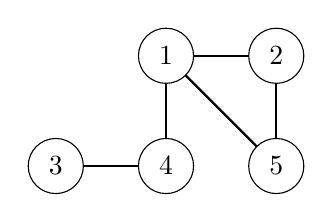
\begin{tikzpicture}[scale=0.7]

\draw ( 2,2) circle (0.5cm);
\draw ( 4,2) circle (0.5cm);
\draw ( 0,0) circle (0.5cm);
\draw ( 2,0) circle (0.5cm);
\draw ( 4,0) circle (0.5cm);

\draw ( 2,2) node{1};
\draw ( 4,2) node{2};
\draw ( 0,0) node{3};
\draw ( 2,0) node{4};
\draw ( 4,0) node{5};

\draw[thick] (0.5,0) -- (1.5,0);
\draw[thick] (2.5,2) -- (3.5,2);
\draw[thick] (2,1.5) -- (2,0.5);
\draw[thick] (4,1.5) -- (4,0.5);
\draw[thick] (2.35355339,1.64644661) -- (3.64644661,0.35355339);

\end{tikzpicture}


  \caption{Esempio di un $5$--cluster.}
  \label{fig:06-5cluster}
\end{figure}
%%%%%%%%%%%%%%%%%%%%%%%%%%%%%%%%%%%%%%%%%%%%%%%%%%%%%%%%%%%%%%%%%%%%%%%%%
Dovrebbe risultare ovvio che un tale cluster non può essere decomposto in cluster più semplici, ovvero che la sua espressione non può essere fattorizzata in integrali indipendenti. Il termine descritto dal cluster in figura \ref{fig:06-5cluster} è infatti
\be
t = \int f_{1,2}f_{1,4}f_{1,5}f_{2,5}f_{3,4}\,\de^3r_1\de^3r_2\de^3r_3\de^3r_4\de^3r_5
\ee
Notiamo anche che un gruppo di $\ell$ particelle (tranne che per $\ell = 1, 2$: infatti gli $1$--cluster e i $2$--cluster sono banali) può portare a un certo numero di $\ell$--cluster, alcuni dei quali avranno un valore uguale. Per esempio, per $\ell = 3$ possiamo ottenere $4$ distinti $3$--cluster, quelli che  troviamo in figura \ref{fig:06-3cluster}.
%%%%%%%%%%%%%%%%%%%%%%%%%%%%%%%%%%%%%%%%%%%%%%%%%%%%%%%%%%%%%%%%%%%%%%%%%
\begin{figure}[h]
  \centering
  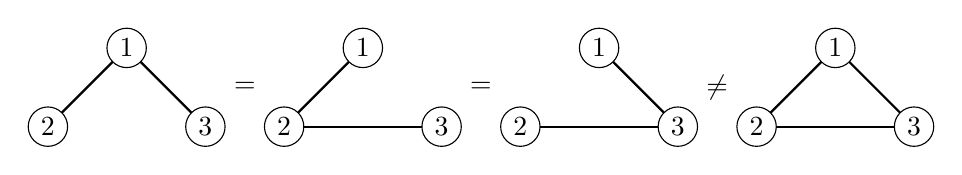
\begin{tikzpicture}[scale=0.5]

\draw ( 0,0) circle (0.5cm);
\draw ( 4,0) circle (0.5cm);
\draw ( 6,0) circle (0.5cm);
\draw (10,0) circle (0.5cm);
\draw (12,0) circle (0.5cm);
\draw (16,0) circle (0.5cm);
\draw (18,0) circle (0.5cm);
\draw (22,0) circle (0.5cm);

\draw ( 2,2) circle (0.5cm);
\draw ( 8,2) circle (0.5cm);
\draw (14,2) circle (0.5cm);
\draw (20,2) circle (0.5cm);

\draw ( 0,0) node{2};
\draw ( 4,0) node{3};
\draw ( 6,0) node{2};
\draw (10,0) node{3};
\draw (12,0) node{2};
\draw (16,0) node{3};
\draw (18,0) node{2};
\draw (22,0) node{3};

\draw ( 2,2) node{1};
\draw ( 8,2) node{1};
\draw (14,2) node{1};
\draw (20,2) node{1};

\draw ( 5,1) node{$=$};
\draw (11,1) node{$=$};
\draw (17,1) node{$\ne$};

\draw[thick] (2.35355339,1.64644661) -- (3.64644661,0.35355339);
\draw[thick] (1.64644661,1.64644661) -- (0.35355339,0.35355339);

\draw[thick] (7.64644661,1.64644661) -- (6.35355339,0.35355339);
\draw[thick] (6.5,0) -- (9.5,0);

\draw[thick] (12.5,0) -- (15.5,0);
\draw[thick] (14.35355339,1.64644661) -- (15.64644661,0.35355339);

\draw[thick] (19.64644661,1.64644661) -- (18.35355339,0.35355339);
\draw[thick] (18.5,0) -- (21.5,0);
\draw[thick] (20.35355339,1.64644661) -- (21.64644661,0.35355339);

\end{tikzpicture}

  \caption{Tutti i possibili $3$--cluster.}
  \label{fig:06-3cluster}
\end{figure}
%%%%%%%%%%%%%%%%%%%%%%%%%%%%%%%%%%%%%%%%%%%%%%%%%%%%%%%%%%%%%%%%%%%%%%%%%

Possiamo introdurre ora l'integrale di cluster $b_\ell$, definito da
\be
b_\ell(V,T) = \dfrac{1}{\ell!\lambda^{3(\ell-1)}V}\sum\left(
{\text{su tutti i possibili $\ell$--cluster}}
\right)
\ee
Questa quantità ci farà comodo in seguito. Per il momento ci limitiamo a notare che nel limite di volume infinito, $b_\ell(V,T)$ tende a un limite, chiamiamolo $\bslash_\ell(T)$, che non dipende dal volume stesso. Per capire questo fatto possiamo immaginare, negli integrali coinvolti nel calcolo di $b_\ell$, di fissare la coordinata $r_1$ e di integrare sulle $(\ell-1)$ coordinate che rimangono. Tutte le $f_{ij}$ coinvolte nell'integrale, come abbiamo visto, sono diverse da zero in un range molto limitato, e il risultato di queste $(\ell-1)$ integrazioni, a parte effetti di bordo che spariscono come termini di superficie quando il volume va a infinito, non possono dipendere dal volume. Infine integriamo sulla coordinata rimasta libera, $r_1$, e otteniamo un esplicito fattore $V$ che si cancella con il $V$ a denominatore nella definizione di $b_\ell(V,T)$. Tutto questo a patto che la forma del contenitore non sia troppo stramba, così che il termine di superficie dato dagli effetti di bordo possa sparire nel limite termodinamico. Vediamo, come esempio, i primi tre coefficienti.
\bea
\label{eq:06-bslash-esempi}
b_1 &=& \dfrac{1}{V}\int \de^3r = 1 \nonumber \\
b_2 &=& \dfrac{1}{2\lambda^3 V}\int f_{1,2}\,\de^3r_1\,\de^3r_2 \simeq \dfrac{1}{2\lambda^3}\int f_{1,2}\,
\de^3r_{1,2} \nonumber \\
    &=& \dfrac{2\pi}{\lambda^3}\int_0^\infty f(r)r^2\,\de r =  \dfrac{2\pi}{\lambda^3}\int_0^\infty
        \left( e^{-u(r)/kT} - 1 \right) r^2\,\de r \nonumber \\
b_3 &=& \dfrac{1}{6\lambda^6 V}\int
( f_{1,2}f_{1,3} + f_{1,2}f_{2,3} + f_{1,3}f_{2,3} + f_{1,2}f_{1,3}f_{2,3} ) \; \de^3 r_1\de^3 r_2\de^3 r_3 \nonumber \\
&\simeq& \dfrac{1}{6\lambda^6} \left[ 3\int f_{1,2}f_{1,3}\;\de r_{1,2}\de r_{1,3}
+ \int f_{1,2}f_{1,3}f_{2,3}\;\de r_{1,2}\de r_{1,3} \right] \nonumber \\
&=& 2b_2^2 + \dfrac{1}{6\lambda^6}\int [\cdots]
\eea
Nella precedente abbiamo usato ovunque la notazione $r_{i,j} \equiv |r_i - r_j|$; i quattro termini nell'integrale che definisce $b_3$ sono i quattro $3$--cluster nella figura \ref{fig:06-3cluster}.

Risulta abbastanza facile capire che un generico grafico a $N$--particelle consisterà in un certo numero $m_1$ di $1$--cluster, un certo numero $m_2$ di $2$--cluster, un certo numero $m_3$ di $3$--cluster e così via. Risulta anche facile capire che il set $\{m_\ell\}$, che rappresenta la scomposizione in $\ell$--cluster di un dato grafico a $N$--particelle, non può essere arbitrario, ma deve soddisfare la condizione
\be
\label{eq:06-mellcond}
\sum_{\ell=1}^N \ell m_\ell = N
\ee
Dovrebbe anche risultare chiaro che un dato set $\{m_\ell\}$ non specifica un singolo grafico a $N$--particelle, ma un gruppo di grafici che sebbene simili sono distinti. Chiamiamo $S\{m_\ell\}$ la somma dei valori dei grafici che compongono questo gruppo, ossia tutti i grafici distinti descritti da un certo set $\{m_\ell\}$; quindi date tutte le definizioni è chiaro che possiamo scrivere
\be
Z_N(V,T) = \sideset{}{'}\sum_{\{m_\ell\}} S\{m_\ell\}
\ee
in cui l'apice sulla somma ci ricorda del vincolo (\ref{eq:06-mellcond}); sempre per le definizioni date, avremo che
\be
S\{m_\ell\} = F\{m_\ell\}\prod_\ell \left(b_\ell \ell! \lambda^{3(\ell-1)}V\right)^{m_\ell}
\ee
in cui $W\{m_\ell\}$ è un peso statistico che conta i modi in cui le $N$ particelle possono essere riarrangiate nel vari $\ell$--cluster. Si può far vedere che
\be
W\{m_\ell\} = N!\prod_\ell\dfrac{1}{m_\ell!(\ell!)^{m_\ell}}
\ee
Mettendo tutto insieme otteniamo
\be
Z_N(V,T) = N!\lambda^{3N}\sideset{}{'}\sum_{\{m_\ell\}}\left\{
\prod_\ell\left[\left( b_\ell V/\lambda^3\right)^{m_\ell}\dfrac{1}{m_\ell!}
\right]
\right\}
\ee
nella quale abbiamo usato
\be
\prod_\ell\left(
\lambda^{3(\ell-1)}
\right)^{m_\ell} = \lambda^{3\sum \ell m_\ell}\prod_\ell\left(
\dfrac{1}{\lambda^2}
\right)^{m_\ell} = \lambda^{3N}\prod_\ell\left(
\dfrac{1}{\lambda^2}
\right)^{m_\ell}
\ee
e infine troviamo, per la funzione di partizione del sistema,
\be
Q_N(V,T) = \sideset{}{'}\sum_{\{m_\ell\}}\left\{
\prod_\ell\left[
\left( b_\ell V/\lambda^3\right)^{m_\ell}\dfrac{1}{m_\ell!}
\right]
\right\}
\ee
Il vincolo (\ref{eq:06-mellcond}) rende molto complicato il calcolo di $Q_N(V,T)$. Possiamo risolvere facilmente il problema passando al formalismo grancanonico. Qui si mostra come a volte è possibile calcolare la funzione di granpartizione senza calcolare prima la funzione di partizione, benché la prima sia definita in termini della seconda.

Scriviamo dunque
\be
\calQ(z,V,T) = \sum_{N=0}^\infty z^N Q_N(V,T)
\ee
e poiché
\be
z^N = z^{{\scriptscriptstyle\sum} \ell m_\ell} = \prod_\ell\left( z^\ell \right)^{m_\ell}
\ee
possiamo scrivere
\be
\calQ(z,V,T) = \sum_{N=0}^\infty \left\{
  \sideset{}{'}\sum_{\{m_\ell\}} \left[
    \prod_\ell\left\{ \left( b_\ell V/\lambda^3\right)^{m_\ell}\dfrac{1}{m_\ell!} \right\}
  \right]
\right\}
\ee
Ma ora vediamo che la somma su tutti i possibili valori di $N$ è tale da eliminare il vincolo dalla somma su $\{m_\ell\}$; in altre parole possiamo sommare su tutti gli $m_\ell$ indipendentemente l'uno dall'altro, e ognuno andrà da $0$ a $\infty$. Quindi
\be
\calQ(z,V,T) = \sum_{m_1, m2\dots = 0}^\infty \left[
\prod_\ell\left\{ \left( b_\ell V/\lambda^3\right)^{m_\ell}\dfrac{1}{m_\ell!} \right\}
\right]
\ee
Intercambiando l'ordine della prima sommatoria con la produttoria otteniamo
\bea
\calQ(z,V,T) &=& \prod_{\ell=1}^\infty \left\{
\sum_{m_\ell=0}^\infty \left[
\left( b_\ell V/\lambda^3\right)^{m_\ell}\dfrac{1}{m_\ell!}
\right]
\right\} \nonumber \\
&=& \prod_{\ell=1}^\infty \exp\left( b_\ell z^\ell V/\lambda^3 \right) = 
\exp\left( \sum_{\ell=1}^\infty b_\ell z^\ell V/\lambda^3  \right)
\eea
Possiamo quindi scrivere
\bea
\label{eq:06-PVNkT}
\dfrac{P}{kT} &=& \lim_{V\to\infty}\left(
\dfrac{1}{V}\ln\calQ
\right) = \dfrac{1}{\lambda^3}\sum_{\ell=1}^\infty \bslash_\ell z^\ell \nonumber \\
n = \dfrac{N}{V} &=&\lim_{V\to\infty}\left(
\dfrac{z}{V}\dpar{\ln\calQ}{z} 
\right) = \dfrac{1}{\lambda^3}\sum_{\ell=1}^\infty \ell \bslash_\ell z^\ell
\eea
Come abbiamo già visto quando abbiamo studiato il formalismo grancanonico, per ottenere l'equazione di stato dobbiamo ottenere la fugacità $z$ in funzione della densità $n$ dalla seconda delle 
(\ref{eq:06-PVNkT}) e sostituire il risultato nella prima. Il problema, in questo caso, è che $n$ è dato come una serie di potenze in $z$: dobbiamo quindi invertire la serie, e quindi ottenere $z$ come una serie di potenze in $n$. L'inversione di una serie di potenze si effettua in maniera iterativa. Prima di tutto scriviamo
\be
n\lambda^3 = \bslash_1 z + 2\bslash_2 z^2 + 3\bslash_3 z^3 + \cdots
\ee
e isoliamo $z$ sul lato sinistro della nuova equazione:
\be
\label{eq:06-inversa}
z = \dfrac{n\lambda^3 - 2\bslash_2 z^2 - 3\bslash_3 z^3 - \cdots}{\bslash_1}
\ee
Otteniamo la soluzione all'ordine $1$ se trascuriamo, nella (\ref{eq:06-inversa}), i termini $O(z^2)$ e superiori. Abbiamo quindi
\be
\label{eq:06-z1}
z^{(1)} = \dfrac{n\lambda^3}{\bslash_1}
\ee
Possiamo ottenere l'equazione di stato all'ordine più basso se sostituiamo questo valore nella prima delle (\ref{eq:06-PVNkT}), con l'accorgimento che dobbiamo dobbiamo, come prima, trascurare i termini $O(z^2)$ e superiori. Si ottiene facilmente $PV = NkT$, ossia l'equazione di stato dei gas ideali (cosa che non è affatto sorprendente ma che ci conforta).

Per ottenere la prima correzione all'equazione di stato occorre andare all'ordine superiore: prendiamo quindi il valore di $z$ fornito dalla (\ref{eq:06-z1}) e inseriamolo nella (\ref{eq:06-inversa}), ricordandoci che stavolta dobbiamo trascurare termini $O(z^3)$ e superiori. Troviamo
\be
z^{(2)} = \dfrac{n\lambda^3 - 2\bslash_2(n\lambda^3)^2/\bslash_1^2}{\bslash_1}
= \dfrac{n\lambda^3}{\bslash_1}\left(
1 - \dfrac{2\bslash_2(n\lambda^3)}{\bslash_1^2}
\right)
\ee
Se portassimo avanti l'inversione della serie, scopriremmo che in realtà stiamo espandendo $z$ in serie di potenze di $n\lambda^3$, e quindi sostituendo questa espansione nella prima delle (\ref{eq:06-PVNkT}) otterremo la quantità $PV/NkT$ come una serie di potenze in $n\lambda^3$. In tutta generalità possiamo scrivere
\be
\dfrac{PV}{NkT} = \sum_{\ell=1}^\infty a_\ell(T) (n\lambda^3)^{\ell-1}
\ee
e quest'ultima equazione è nota con il nome di {\em espansione del viriale}. I coefficienti $a_\ell$ possono essere calcolati iterativamente come abbiamo mostrato prima, e troviamo
\bea
a_1 &=& \bslash_1 = 1 \nonumber \\
a_2 &=& -\bslash_2 = -\dfrac{2\pi}{\lambda^3}\int_0^\infty \left( 
e^{-u(r)/kT} - 1 
\right) r^2\,\de r \nonumber\\
a_3 &=& 4\bslash_2^2 - 2\bslash_3 = 4\bslash_2^2 - 2\left(
2\bslash_2^2 + \dfrac{1}{6\lambda^6}\int f_{1,2}f_{1,3}f_{2,3}\,\de^3 r_{1,2}\,\de^3 r_{1,3}
\right) \nonumber \\
&=& -\dfrac{1}{3\lambda^6}\int[\cdots]
\eea
Mentre i primi due coefficienti del viriale sono banali, notiamo che il terzo dipende solo dall'unico $3$--cluster {\em irriducibile}, ossia il quarto a destra nella figura \ref{fig:06-3cluster}. Un $\ell$--cluster irriducibile è un$\ell$--cluster che non può essere decomposto in due $\ell$--cluster separati eliminando una sola linea (è evidente, per esempio, che gli altri tre cluster nella figura \ref{fig:06-3cluster} sono riducibili). Si può dimostrare che questa proprietà del terzo coefficiente del viriale vale anche a tutti gli ordini superiori, ossia che il coefficiente $a_\ell$ dipende solo dagli $\ell$--cluster irriducibili.

Questo fatto costituisce una formidabile analogia con l'espansione in potenze della costante d'accoppiamento delle teorie di campo quantistiche e relativistiche: in questo caso infatti si può mostrare che occorre calcolare solo diagrammi di Feynman {\em one--particle--irreducible}, ossia diagrammi che, una volta eliminate tutte le gambe asintotiche esterne, non possono essere spezzati in sottodiagrammi indipendenti tagliando un solo propagatore.

\subsection{L'equazione di van der Waals}

Calcoliamo ora il secondo coefficiente del viriale nel caso di un potenziale semplificato. Per la parte repulsiva consideriamo le particelle come sfere rigide, quindi un potenziale infinito sotto una certa distanza $r_0$, mentre la parte attrattiva la prendiamo uguale al potenziale di Lennard-Jones:
\be
u(r) = \left\{
\begin{array}{ll}
\infty & \textrm{se\ } r < r_0 \\
-u_0(r_0/r)^6 & \textrm{se\ } r \ge r_0
\end{array} \right.
\ee
In questo caso abbiamo
\be
a_2 = \dfrac{2\pi}{\lambda^3}\left[
\int_0^{r_0} r^2\,\de r + \int_{r_0}^\infty \left\{
1 - \exp\left( \dfrac{u_0}{kT}(r_0/r)^6\right)
\right\}r^2\,\de r
\right]
\ee
Nel secondo integrale assumiamo che valga $u_0/kT(r_0/r)^6 \ll 1$, ed espandiamo l'esponenziale. Otteniamo quindi
\be
a_2 = \dfrac{2\pi}{3\lambda^3}r_0^3\left( 1 -\dfrac{u_0}{kT} \right)
\ee
Un po' di manipolazioni algebriche ci portano al risultato cercato, ossia l'equazione di van der Waals:
\be
\left( P + \dfrac{a}{v^2} \right)(v - b) = kT
\ee
a patto di identificare
\bea
a &=& \dfrac{2\pi r_0^3 u_0}{3} \nonumber \\
b &=& \dfrac{2\pi r_0^3}{3}
\eea
Notiamo che il risultato per $b$ è esattamente lo stesso che avevamo ottenuto nell'esercizio \ref{ex:02-sfere}. Occorre considerare infatti che $r_0$ è la distanza di minimo avvicinamento tra due particelle, e quindi sostanzialmente il doppio del ``raggio effettivo'' di una particella.

%%%%%%%%%%%%%%%%%%%%%%%%%%%%%%%%%%%%%%%%%%%%%%%%%%%%%%%%%%%%%%%%%%%%%%

\vskip 0.75cm
\begin{flushright}
{\em Ultimo aggiornamento del Capitolo: 22.04.2017}
\end{flushright}
